% This is "sig-alternate.tex" V2.1 April 2013
% This file should be compiled with V2.5 of "sig-alternate.cls" May 2012
%
% This example file demonstrates the use of the 'sig-alternate.cls'
% V2.5 LaTeX2e document class file. It is for those submitting
% articles to ACM Conference Proceedings WHO DO NOT WISH TO
% STRICTLY ADHERE TO THE SIGS (PUBS-BOARD-ENDORSED) STYLE.
% The 'sig-alternate.cls' file will produce a similar-looking,
% albeit, 'tighter' paper resulting in, invariably, fewer pages.
%
% ----------------------------------------------------------------------------------------------------------------
% This .tex file (and associated .cls V2.5) produces:
%       1) The Permission Statement
%       2) The Conference (location) Info information
%       3) The Copyright Line with ACM data
%       4) NO page numbers
%
% as against the acm_proc_article-sp.cls file which
% DOES NOT produce 1) thru' 3) above.
%
% Using 'sig-alternate.cls' you have control, however, from within
% the source .tex file, over both the CopyrightYear
% (defaulted to 200X) and the ACM Copyright Data
% (defaulted to X-XXXXX-XX-X/XX/XX).
% e.g.
% \CopyrightYear{2007} will cause 2007 to appear in the copyright line.
% \crdata{0-12345-67-8/90/12} will cause 0-12345-67-8/90/12 to appear in the copyright line.
%
% ---------------------------------------------------------------------------------------------------------------
% This .tex source is an example which *does* use
% the .bib file (from which the .bbl file % is produced).
% REMEMBER HOWEVER: After having produced the .bbl file,
% and prior to final submission, you *NEED* to 'insert'
% your .bbl file into your source .tex file so as to provide
% ONE 'self-contained' source file.
%
% ================= IF YOU HAVE QUESTIONS =======================
% Questions regarding the SIGS styles, SIGS policies and
% procedures, Conferences etc. should be sent to
% Adrienne Griscti (griscti@acm.org)
%
% Technical questions _only_ to
% Gerald Murray (murray@hq.acm.org)
% ===============================================================
%
% For tracking purposes - this is V2.0 - May 2012

\documentclass{sig-alternate-05-2015}
\usepackage{graphicx}
\usepackage{epstopdf} %converting to PDF
\usepackage{xspace}
\usepackage{enumitem}
\usepackage{svg}
\usepackage[ruled,linesnumbered]{algorithm2e}
\usepackage{subfig}
\usepackage{adjustbox}
\usepackage{wrapfig}
%\usepackage{lipsum}
\usepackage{graphbox}
%\usepackage{tabularx}
%\usepackage[linesnumbered]{algorithm2e}
%\usepackage[linesnumbered,ruled]{algorithm2e}
%\usepackage[linesnumbered,ruled,vlined]{algorithm2e}
\begin{document}
%\setcopyright{acmcopyright}
\setcopyright{none}
%\setcopyright{acmlicensed}
%\setcopyright{rightsretained}
%\setcopyright{usgov}
%\setcopyright{usgovmixed}
%\setcopyright{cagov}
%\setcopyright{cagovmixed}


% DOI
%\doi{10.475/123_4}

% ISBN
%\isbn{123-4567-24-567/08/06}
%
%Conference
%\conferenceinfo{PLDI '13}{June 16--19, 2013, Seattle, WA, USA}

%\acmPrice{\$15.00}

%
% --- Author Metadata here ---
%\conferenceinfo{WOODSTOCK}{'97 El Paso, Texas USA}
%\CopyrightYear{2007} % Allows default copyright year (20XX) to be over-ridden - IF NEED BE.
%\crdata{0-12345-67-8/90/01}  % Allows default copyright data (0-89791-88-6/97/05) to be over-ridden - IF NEED BE.
% --- End of Author Metadata ---

%\title{Alternate {\ttlit ACM} SIG Proceedings Paper in LaTeX
%Format\titlenote{(Produces the permission block, and
%copyright information). For use with
%SIG-ALTERNATE.CLS. Supported by ACM.}}
\title{Automatic Inference of Application Reputation via PageRank on System Monitoring Data}
%\subtitle{[Extended Abstract]
%\titlenote{A full version of this paper is available as
%\textit{Author's Guide to Preparing ACM SIG Proceedings Using
%\LaTeX$2_\epsilon$\ and BibTeX} at
%\texttt{www.acm.org/eaddress.htm}}}
%
% You need the command \numberofauthors to handle the 'placement
% and alignment' of the authors beneath the title.
%
% For aesthetic reasons, we recommend 'three authors at a time'
% i.e. three 'name/affiliation blocks' be placed beneath the title.
%
% NOTE: You are NOT restricted in how many 'rows' of
% "name/affiliations" may appear. We just ask that you restrict
% the number of 'columns' to three.
%
% Because of the available 'opening page real-estate'
% we ask you to refrain from putting more than six authors
% (two rows with three columns) beneath the article title.
% More than six makes the first-page appear very cluttered indeed.
%
% Use the \alignauthor commands to handle the names
% and affiliations for an 'aesthetic maximum' of six authors.
% Add names, affiliations, addresses for
% the seventh etc. author(s) as the argument for the
% \additionalauthors command.
% These 'additional authors' will be output/set for you
% without further effort on your part as the last section in
% the body of your article BEFORE References or any Appendices.

\numberofauthors{3} %  in this sample file, there are a *total*
% of EIGHT authors. SIX appear on the 'first-page' (for formatting
% reasons) and the remaining two appear in the \additionalauthors section.
%
\author{
% You can go ahead and credit any number of authors here,
% e.g. one 'row of three' or two rows (consisting of one row of three
% and a second row of one, two or three).
%
% The command \alignauthor (no curly braces needed) should
% precede each author name, affiliation/snail-mail address and
% e-mail address. Additionally, tag each line of
% affiliation/address with \affaddr, and tag the
% e-mail address with \email.
%
% 1st. author
\alignauthor
Pengcheng Fang\\
       \affaddr{Case Western Reserve University}\\
%       \email{pxf109@case.edu}
% 2nd. author
\alignauthor
Xusheng Xiao\\
       \affaddr{Case Western Reserve University}\\
%       \email{xusheng.xiao@case.edu}
% 3rd. author
\alignauthor Lingming Zhang\\
       \affaddr{University of Texas at Dallas}\\
%       \affaddr{Brookhaven National Lab}\\
%       \affaddr{P.O. Box 5000}\\
%       \email{lleipuner@researchlabs.org}
% 5th. author
%\alignauthor Sean Fogarty\\
%       \affaddr{NASA Ames Research Center}\\
%       \affaddr{Moffett Field}\\
%       \affaddr{California 94035}\\
%       \email{fogartys@amesres.org}
% 6th. author
%\alignauthor Charles Palmer\\
%       \affaddr{Palmer Research Laboratories}\\
%       \affaddr{8600 Datapoint Drive}\\
%       \affaddr{San Antonio, Texas 78229}\\
%       \email{cpalmer@prl.com}
}
% There's nothing stopping you putting the seventh, eighth, etc.
% author on the opening page (as the 'third row') but we ask,
% for aesthetic reasons that you place these 'additional authors'
% in the \additional authors block, viz.
%\additionalauthors{Additional authors: John Smith (The Th{\o}rv{\"a}ld Group,
%email: {\texttt{jsmith@affiliation.org}}) and Julius P.~Kumquat
%(The Kumquat Consortium, email: {\texttt{jpkumquat@consortium.net}}).}
%\date{16 April 2018}
% Just remember to make sure that the TOTAL number of authors
% is the number that will appear on the first page PLUS the
% number that will appear in the \additionalauthors section.

\maketitle
\input{Abstract}


%
% The code below should be generated by the tool at
% http://dl.acm.org/ccs.cfm
% Please copy and paste the code instead of the example below. 
%
%\begin{CCSXML}
%<ccs2012>
% <concept>
%  <concept_id>10010520.10010553.10010562</concept_id>
%  <concept_desc>Computer systems organization~Embedded systems</concept_desc>
%  <concept_significance>500</concept_significance>
% </concept>
% <concept>
%  <concept_id>10010520.10010575.10010755</concept_id>
%  <concept_desc>Computer systems organization~Redundancy</concept_desc>
%  <concept_significance>300</concept_significance>
% </concept>
% <concept>
%  <concept_id>10010520.10010553.10010554</concept_id>
%  <concept_desc>Computer systems organization~Robotics</concept_desc>
%  <concept_significance>100</concept_significance>
% </concept>
% <concept>
%  <concept_id>10003033.10003083.10003095</concept_id>
%  <concept_desc>Networks~Network reliability</concept_desc>
%  <concept_significance>100</concept_significance>
% </concept>
%</ccs2012>  
%\end{CCSXML}

%\ccsdesc[500]{Computer systems organization~Embedded systems}
%\ccsdesc[300]{Computer systems organization~Redundancy}
%\ccsdesc{Computer systems organization~Robotics}
%\ccsdesc[100]{Networks~Network reliability}


%
% End generated code
%

%
%  Use this command to print the description
%
%\printccsdesc

% We no longer use \terms command
%\terms{Theory}

\keywords{System Monitoring; GraphSplit; Dependency Graph}

\section{Introduction}
Advanced Persistent Threat (APT) attacks~\cite{fireeye:anatomy,aptsymantec} have caused many well-protect firms with significant financial\\ losses~\cite{ebay,opm,target,homedepot} and become the reason for people and companies seek safer and more comprehensive information security protections. Yahoo data breach leaked over 1 billion accounts' sensitive information. This security event caused Verizon to cut the price of the deal with Yahoo by 350 million~\cite{ya:yahooleak,aptsymantec}. These APT attacks often consist of many individual attack steps across many hosts and leverage advanced tools and malware to penetrate into an enterprise~\cite{fireeye:anatomy,aptsymantec}. These complex strategies and customized tools make APT hard to be prevented. Even though these attacks can be powerful and stealthy, one typical constrains from the attacker side is that such an attack consisted by multiple steps could leave the multiple attack footprints as ``dots''.

In order to achieve the version of connecting the dots, the first challenge is to collect and store the dots. This goal can be achieved by the system kernel listening tool which can gather and output the information of system calls and provides a comprehensive way to capture system behaviors~\cite{backtracking,backtracking2}. Unlike its alternatives (file accesses, firewall and network monitoring) that provide partial  information and are application-specific, system monitoring covers all activities among system entities(process, files, sockets, and pipes) over time, providing a global view of system activities.

The second challenge for achieving the vision of connecting the dots is to connect dots even interleaved with multiple system activities. The state-of-art~\cite{taser,backtracking,backtracking2} techniques take processes as subjects and other system entities as objects. System call events happen between system entities establish edges between subjects and objects. If an anomalous is detected, a dependency analysis is applied to  connected system call events via causality. In order to finish the dependency analysis quickly, an efficient design storage and index of log data is necessary.However, APT attacks could remain stealthy for more than half a year~~\cite{trustwave}, and monitoring attack provenance on every host in an enterprise for such a period of time (\url{~}0.5--1.0 GB per host per day) is burdensome and laborious. Therefore, gathering and storing data for dependency analysis in an enterprise is an daunting task. To mitigate the problem of overwhelmingly big-data of attack derived from system monitoring data for dependency analysis, the Backtracking and Causality Preserved Reduction (CPR) are applied to shrink the size of dependency graph.

The logistics behind the Backtracking is that the events that happened after the anomalous event can not be part of multiple attack steps of APT, and therefore these events can be removed from the dependency graph. The insight of Causality Preserved Reduction is that some events have identical dependency impact space (same subject and same objects), and therefore they can be safely aggregated.

The third challenge is that although dependency analysis reveals the causality of an anomalous event as a dependency graph, they only scratch the surface of how causality analysis can be used to enhance the defense of APT attacks: it is still slow and laborious for security analysts to filter unrelated events and recover the attack sequence from the large dependency graph. In APT attacks, many steps require downloading and installing customized applications and libraries to enterprise system to succeed, such as malware injection and privilege escalation~\cite{apt,aptmalware,defendapt} and blocking applications and libraries from entering the enterprises can counter these attacks. 
%However, existing techniques that reject software with unseen signatures are ineffective in blocking malicious software installation, since they would also reject many user's application installations that adopts a faster delivery cycle for including patches and new features. 
In this project, PageRank~\cite{pagerank} is used to infer reputation of all system entities. The libraries or applications from unknown source has lower reputation compared with those from reliable channels, such as Google, Apple, Samsung and so on. After that, we can reconstruct steps based on each entity's reputation.
\section{Background}
\subsection{System Monitoring}
System monitoring data consists of various system activities in the form of events along with time~\cite{backtracking, backtracking2, taser,wormlog}. Each event can naturally be described as a system entity (subject) does some operation on another system entity(object). For example, a process reads a file or a process accesses a network connection. An APT attack needs multiple step to succeed , such as target discovery and data exfiltration, as illustrated in the cyber kill chain\cite{killchain}. Therefore, multiple attack footprints might be left as "dots", which can be captured precisely by system monitoring. System monitoring data for Windows and Linux can be collected via ETW event tracing\cite{etw} and Linux Audit Framework\cite{auditd}. The audit framework used in this project is a popular and opensource audit application: Sysdig.
\begin{figure}
	\centering
	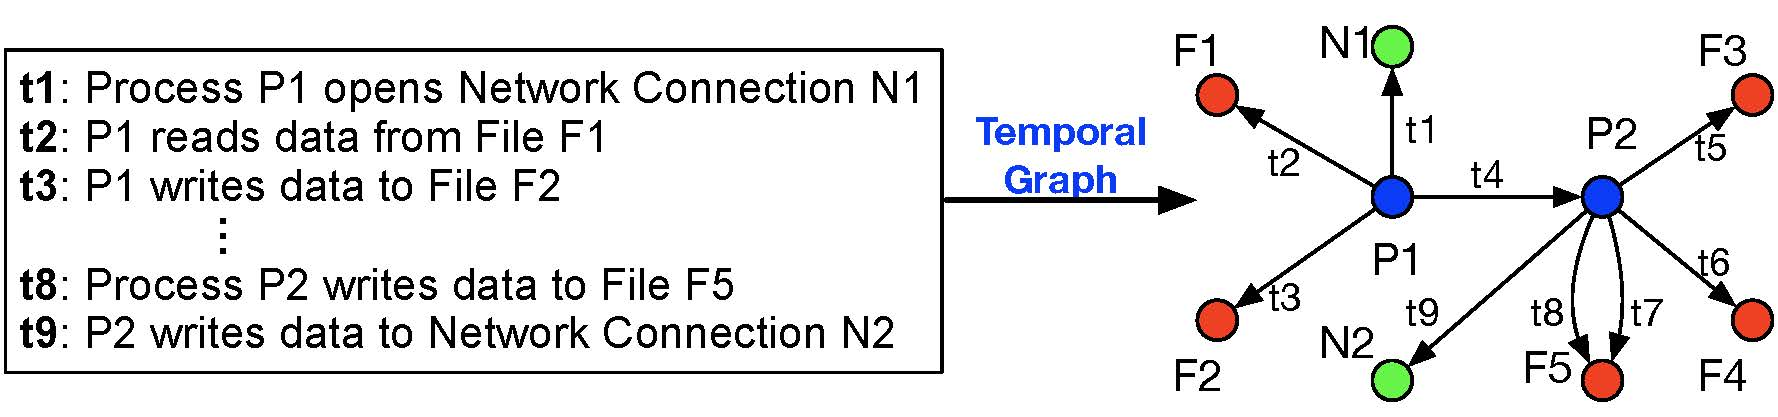
\includegraphics[width=0.48\textwidth]{temporal-graph.jpg}
	\caption{System monotoring Data}
	\label{fig:temporalGraph}
\end{figure}
\subsection{Sysdig}
Sysdig is a popular system and container monitoring tool. It improve the system and container visibility, combined with Kubernetes, Docker and Mesos integration, better record enterprises's services. It gives system manager an easy access to the actual behavior of the system and container. Far too often, system-level monitoring still involves logging into a machine with SSH and using plethora of dated tools with very inconsistent interfaces. Sysdig instruments physical and virtual machine at the operating system level by installing into the Linux kernel and capturing system calls and other system events.
\subsection{Output data description}
\begin{figure}[h]
	\centering
	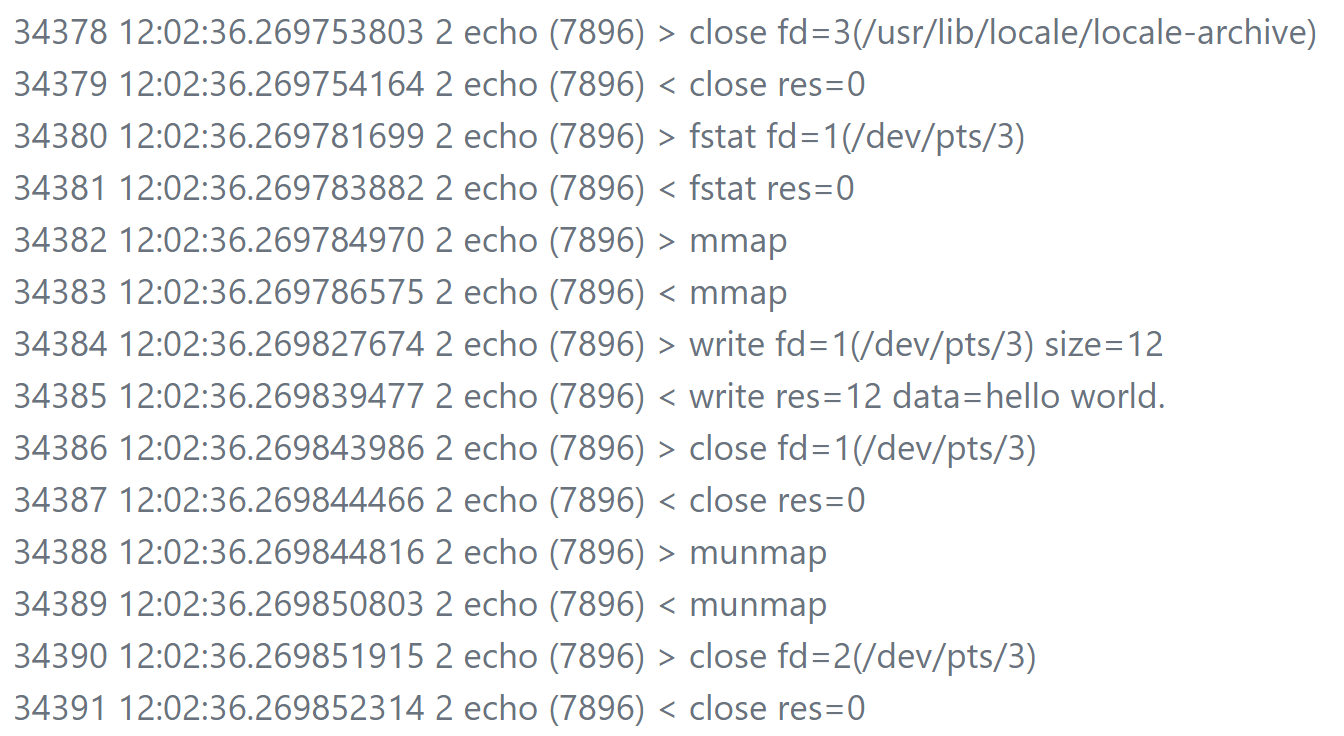
\includegraphics[scale=0.5]{fig1}
	\caption{Raw Data Output}
\end{figure}
The raw output data already includes many useful information, however it is still not enough to build the dependency graph of all the system behaviors. According to the Sysdig user guide, the output data format is defined as: 
\vspace{0.2em}

\noindent{\texttt{\%evt.num \%evt.rawtime.s.\%evt.rawtime.ns \%evt.cpu \\ \%proc.name (\%proc.pid) \%evt.dir \%evt.type cwd=\%proc.cwd \%evt.args latency=\%evt.latency}}

where:
\begin{itemize}[noitemsep]
	\item evt.num is the incremental event number.
	\item evt.rawtime.s is second part of the event timestamp.
	\item evt.rartime.na is nanosecond part of the event timestamp.
	\item evt.cpu is the CPU number where the event was captured
	\item proc.name is the name of the process that generated the event.
	\item proc.pid is the process id that generated the event
	\item evt.dir is the event direction, > for enter events < for exit events.
	\item evt.type is the name of system event e.g. 'open' or 'read'.
	\item proc.cwd is the current working directory of the event.
	\item evt.args is all the event agruments, aggregated into a single string.
	\item evt.latency is the delta between an exit event and the correspondent enter event in nanoseconds.
\end{itemize}
\begin{figure}
	\centering
	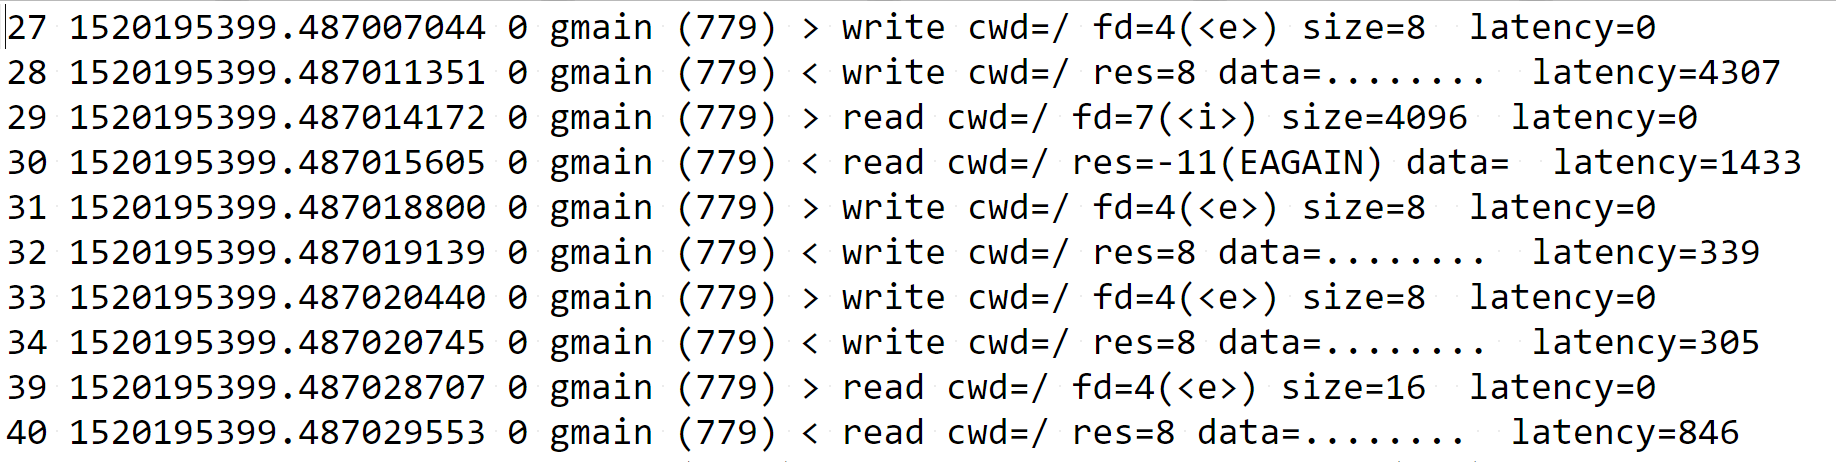
\includegraphics[scale=0.4]{fig2}
	\caption{Self-defined Data format}
\end{figure}
Currently, the information we try to gather includes events start time ,exit time, the id and name of the process that generated the event, the event arguments and duration. Based on the observation, the output data also includes many \textit{switch} events, which is generated by the CPU task scheduling algorithm. This information is too detail and unnecessary for the dependency graph analysis. The goal of system monitoring is to record the legal user's or unknown attacker's operation. Therefore, this  kind event can be safely neglected. In this project, there are three type system events need to be processed. The first type is about how a process is created. The relevant events are clone and fork in Linux system. The second type is file operations. The relevant event about this type are read, write and writev. The third type event is about network communication. The relevant system events are sendto. Through the filter provided by Sisdig, we can only gather the interested events.
%\subsection{Log Parser}
%After gathering the data, we need build the dependency graph based on the log file. There are three type vertexes representing three kind system entities: process, file and network communication.
%The identifier for process is its name and id.  For file, it is identified by its absolute file path, for network communication, it is distinguished by the communication two sides' ip and port number. We use three kind shape to represent these three system entities. According to the entities included in the system event, the parser need to process five kinds edge : process to process, process to file, file to process, network to process, process to network. The type of edge is decided by the event arguments. The output of Sysdig will use \textit{fd} as its identifier or key word. In the value part, it will use different characters to represent different objects.For example, it use \textit{f} to represent file, \textit{6} to represent IPV6 sockets,\textit{4} to represent IPV4 sockets. This kind information is necessary, without this, it is hard to know the start or end of information flow is a file or an ip address.  Through this way, the parser can know the kind of entities generating this event. For process to process event, we can directly know objects generating this event is two processes, because its event type is unique : fork or clone. In the conclusion, the parser will establish the dependency relationship between two system entities. This dependency relationship is specified by three parts: a source object, a sink object and a time interval$(t_s(e), t_e(e))$
\subsection{Dependency Anlysis}
Dependency analysis~\cite{backtracking,backtrackingfile,backtracking2} plays an important role in security applications,
such as finding the entry points of attacks (\emph{causal analysis})
and investigating ramification of attacks (\emph{impact analysis}).
Given events $evt_1$ and $evt_2$, to construct a backward (forward) dependency $evt_1\xrightarrow{backward} evt_2$ ($evt_1\xrightarrow{forward} evt_2$), $evt_1$ must occur after (before) $evt_2$.

Backward dependency analysis can be used to analyze the \emph{causality} of an anomalous event,
such as the creation of an unknown executable in a system.
%Nowadays, executables in a computer are frequently updated, and thus not all malicious ones may be captured by anti-virus software. 
%To know whether an executable is safe to run, it is important to know whether it comes from trusted sources, such as Windows updates or official updaters like the Chrome updater.
Backward dependency analysis finds the origins of the executables by searching the events backward in time: 
(1) start the investigation of the processes that create the executables;
(2) from the processes, trace back to see which executables the processes executed;
(3) if the executables are from a trusted source, then we can stop the search; 
otherwise, the tracking continues until it finds the origin (such as installer files or downloaders).
As another example, forward dependency analysis helps users understand the ramification of malware.
Assume that we identified a malicious script in the web server. 
To understand how it infects a victim machine, we can start the investigation of the process that executed or read from the script,
and trace whether they propagate the malicious scripts across hosts
In this project, the goal of this step is to reconstruct the time line in an attack.
However, modern operation system is very complex, even through the user does not do any specific operation, it still has many service process running at the backend. That will generate many log records in the audit tool's output. In other words, these events will be represented as many edges and vertexes that we don't need. So we need to run backtrack\cite{backtracking, backtracking2} from at least one \textit{detection point}\cite{lamport1978time}, such as a modified, extra, or deleted file, or a suspicious or missing process. There are two standards to decide which system entity or operation is relevant to \textit{detection point} or not. The first one is whether there is a path existing between two vertexes or not. That means the source entity can use several operations to affect the state of the object entity. The second one is that the time intervals can be used to reduce false dependencies. For example, a process that reads a file at time 10 does not depend on writes to the file that that occur after time 10. The figure in the first column of Fiture~\ref{fig:backandCPR} is the dependency reconstruction about how a python script read data from source file and then write data to another file. It is not hard to notice there are multiple edge existing between the same pair of vertexes. It gives us ground to further reduce the size of this dependency graph.
%\begin{figure}[!htbp]
%	\centering
%	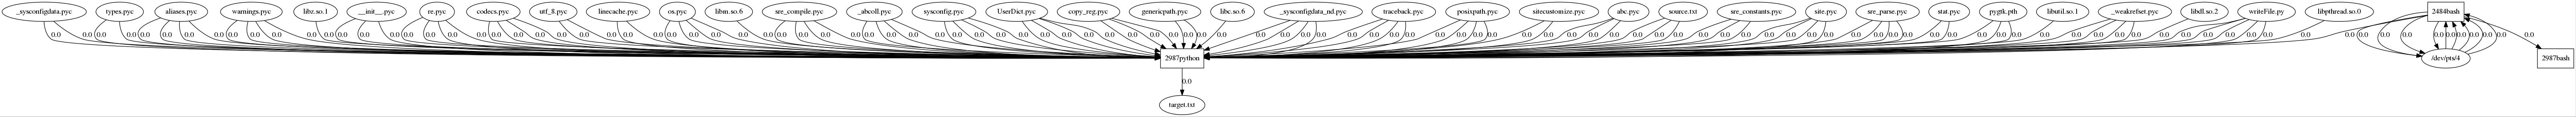
\includegraphics[width=1.3\textwidth,angle=90]{fileBack.jpg}
%	\caption{Backtracking of File operation}
%	\label{fig:backtrack}
%\end{figure}
\subsection{Causality Preserve Reduction}
From the graph processed by the Backtrack, it is not hard to notice that there are always multiple edges between the same pair of vertexes. This is because the number of operations is not equal to the log record number. For example, If one user try to read a file, the system will not read all data from disk at one time, it will read it hundreds or thousands times. In other words, many edges are corresponding to the same event. In a real-world scenario, an average desktop computer produces more than 1 million events per day, while a server could yield 10 to 100 times the volume. 
%Each day, a rather small system of 100 computers generated more than 200 million events, which requires mid- to high-end server to process and produces databases over 200GB. 
Reducing the data volume is key to solving the scalability problem. Comparing the first and second column of Fiture~\ref{fig:backandCPR}, there is no more duplicate edges between the same pair of vertexes.
%\begin{figure}[!htbp]
%	\centering
%	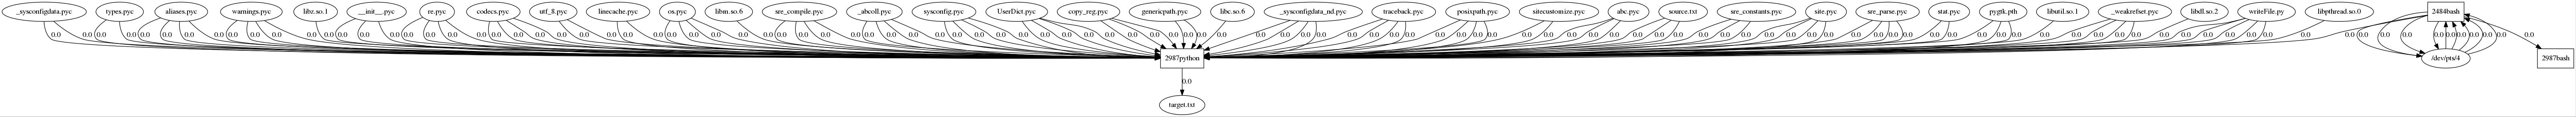
\includegraphics[width=1.3\textwidth,angle=90]{fileBack.jpg}
%	\caption{Backtracking of File operation}
%	\label{fig:CPR}
%\end{figure}
%\begin{figure*}[!hp]
%	\centering
%	\subfloat[Backtracking]{
%		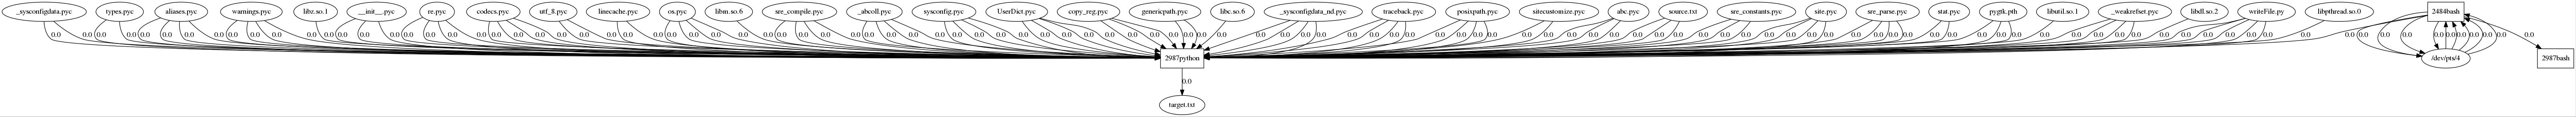
\includegraphics[align=c,width=1.3\textwidth, angle=90]{fileBack.jpg}}
%	\vfill
%	\subfloat[Causality Preserve Reduction]{
%		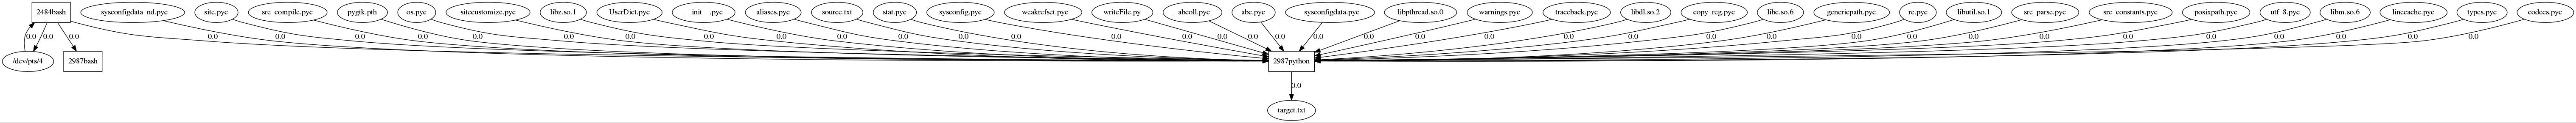
\includegraphics[align=c, width=1.3\textwidth,angle=90]{fileCPR.jpg}}
%\end{figure*}
\begin{figure}[htbp]
	\begin{minipage}[t][0.8\textheight]{0.5\textwidth}
		\centering
		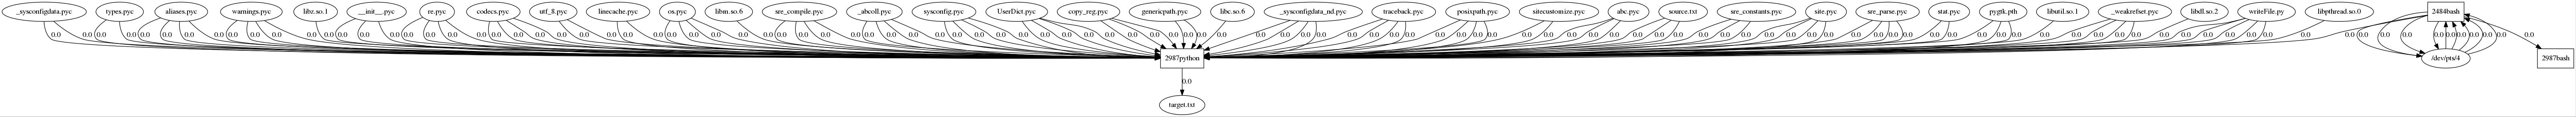
\includegraphics[align=c, width=\textheight,angle=90]{fileBack.jpg}
		\hspace{0.1\textwidth}
		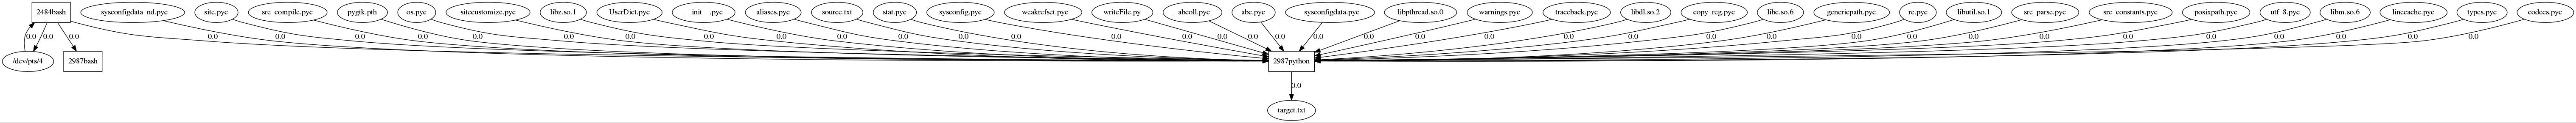
\includegraphics[align=c, width=\textheight,angle=90]{fileCPR.jpg}
	\end{minipage}
	\caption{Backtracking And Causality Preserve Reduction Result}
	\label{fig:backandCPR}
\end{figure}

%\begin{figure}[!htp]
%	\centering
%	\begin{minipage}{0.25\textwidth}
%		\centering
%		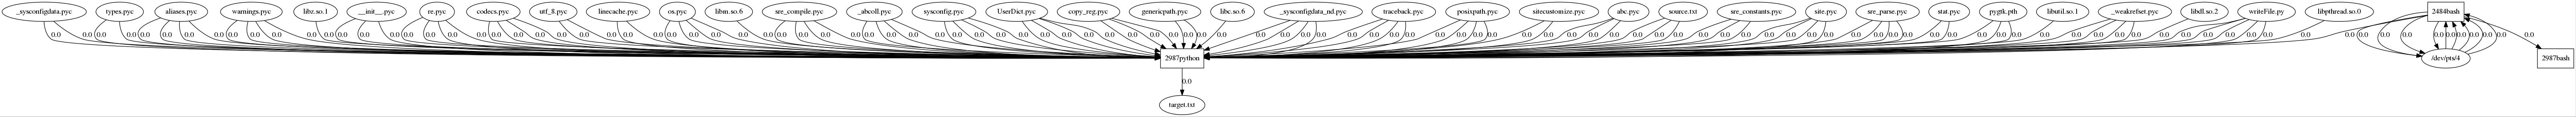
\includegraphics[align=c,width=\textheight, angle=90]{fileBack.jpg}
%		\caption{Backtracking}
%	\end{minipage}
%	\begin{minipage}{0.25\textwidth}
%				\centering
%				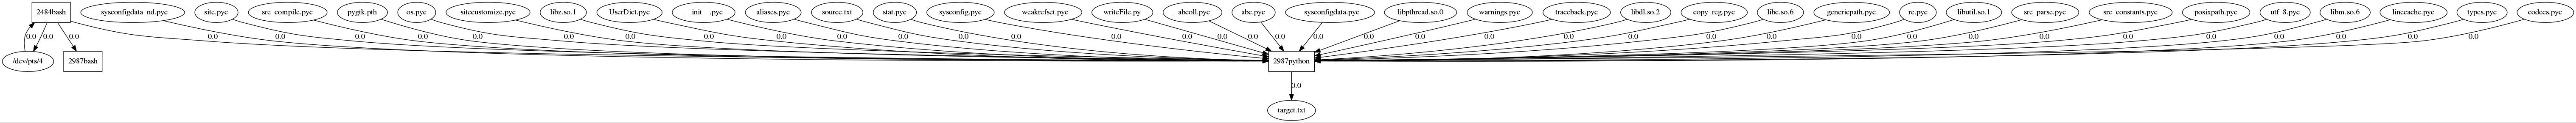
\includegraphics[align=c,width=\textheight, angle=90]{fileCPR.jpg}
%				\caption{CPR}
%	\end{minipage}
%\end{figure}

%While data reduction is a well-studies topic, the most commonly used techniques, spatial and temporal sampling, are not applicable to dependency analysis based on system event traces. Because sampling techniques do not have the inherit concept of causal relations, they are prone to introducing random causal errors. 

\subsubsection{Design}
In this section,  we first present a formal definition of important terms and concepts used in our design.
First, two events have \textit{causality dependency} with each other if an event has information flow that affect the other event.\\
DEFINITION 1: \textbf{Causality Dependency} \\
\indent For two event edges $e_1 = \mathit{(u_1, v_1)} $ and $e_2 = \mathit{(u_2, v_2)} $ , they have causality dependency, if
\begin{itemize}[noitemsep]
	\item $v_1 = u_2 $
	\item $te\mathit{(e_1)} < te\mathit{(e_2)}$
\end{itemize}
if $e_1$ has information flow to $e_2$ and $e_2$  has information flow to $e_3$, then $e_1$ and $e_3$ have causality dependency.
Our primary reduction scheme aims at preserving causality dependency while performing the data reduction. For example, assuming there are multiple edges between the vertex $u$ and $v$, we need to check whether the merge of edges will break the backward trackability and forward trackability~\cite{xu2016high}.We can merge the edges, if that merge will not loss the information about causality dependency.

%\subsection{Graph Split}
% PageRank~\cite{pagerank} considers the World Wide Web as a set of linked nodes and ranks them based on their importance. The insight of PageRank is that a node linked by important nodes should be more important than the ones linked by uninfluenced nodes. That is, a web page's "reputation" is impacted by all the other web pages pointing to it. PageRank uses a transition matrix to represent the weights of edges from node \textit{j} to node \textit{i}. However,although Causality Preserve Reduction can merge many edges, there still may have multiple edges existing the same pair of nodes, because we don't want that the dependency relationship is lost during Causality Preserve Reduction. Therefore, we borrow the idea of static single assignment from(SSA)~\cite{nielson2004principles}, splitting source node  into multiple nodes, where each of the split node has only one outgoing edge pointing to target node. We need duplicate all the edges originally pointing to source to each of the split node from node j.By replacing source node with the split nodes, we can then use PageRank to compute system entities' reputation.\\
% The basic idea for GraphSplit is that for every vertex$(V)$ of the dependency graph, we need to check its incoming edges. If several incoming edges share the same source, we declare a \textit{vertexPair} contains object $V$, source $S$ and a list of edges that connect these two vertexes. We maintain a queue for all $vertexPairs$. We also maintain a set of vertex has alread been  split.If we find the current $vertexPair.S$ or $vertexPair.V$ is split, then we just skip it in current round. We will split it in the next round. Here is the relvant function of GraphSplit.\clearpage
% \begin{algorithm}
%	\caption{GraphSplit}
%	\KwIn{A dependency Graph}
%	\SetKwFunction{FindPair}{FindPair}
%	\SetKwFunction{UpdateGraph}{UpdateGraph}
%	\SetKwFunction{RecoverTimeLogic}{RecoverTimeLogic}
%	\textbf{function}: GraphSplit$(\textit(G))$\\
%	$Queue$ $\leftarrow$ \FindPair{$G$}\;
%	\While{Queue is not Empty}{
%		$V$ $\leftarrow$ $Queue.poll()$\;
%		$S \leftarrow V.source$\;
%		$T \leftarrow V.target$\;
%		\If{Set contains S $or$ Set contains T}{continue}
%		$list1 \leftarrow$ list of outgoing edges of $S$ whose object is not $T$\;
%		$list2 \leftarrow$ V.list\;
%		\UpdateGraph($G$,$list1$,$list2$)\;
%		add $S$ to Set\;
%		$Queue \leftarrow$ \FindPair($G$)\;
%		}
%	\RecoverTimeLogic{$Set$}\;	
%\end{algorithm}
%\begin{algorithm}
%	\caption{FindPair}
%	\KwIn{A dependency Graph(G)}
%	\KwResult{A queue containing the vertex pair need to be splited}
%	\textbf{function}: FindPair$\textit(G)$\\
%	$V \leftarrow G.vertexSet$\;
%	\For{$v \in V$}{
%		$E \leftarrow$ incoming edges of $v$\;
%		\If{$\exists e \in E$ sharing the same source}{
%			$vertexPair.source \leftarrow e.source$\;
%			$vertextPair.object \leftarrow v$\;
%			$vertexPair.object.list$ add $e$\; 
%			$Queue$ add $vertexPair$\;}
%		}
%	\Return{Queue}
%\end{algorithm}
%\begin{algorithm}
%	\caption{RecoverTimeLogic}
%	\KwIn{A set of splited vertex}
%	\textbf{function}: RecoverTimeLogic$\textit(Set)$\\
%	$V \leftarrow G.vertexSet()$\;
%	\For{$v \in V$}{
%		\If{$v$ is the splitting node belongs to $Set$}{
%			$endtime \leftarrow$ the biggest endtime of outgoing edges of $v$\;
%			\For{$e \in$ incoming edges of v}{
%				\If{$e.start > endtime$}{remove this edge\;
%				}
%			}
%		}
%	} 	
%\end{algorithm}
%\begin{algorithm}
%	\caption{UpdateGraph}
%	\KwIn{A dependency Graph and.\\
%		 list1 is a list of outgoning edges of the source except edges whose object is V. \\
%		 list2 is a list containing edges between S and V}
%	\textbf{function}: UndateGraph$\textit(G, list1, list2)$\\
%	$list \leftarrow$ empty list of vertex\;
%	\For{$ e \in list2$}{
%		$u \leftarrow split(S)$\;
%		$list$ add $u$\;
%		$G$ add $u$\;
%		$G$ add a new edge from $u$ to $V$\;
%		}
%	\For{$u \in list$}{
%		\For{$e \in list1$}{
%			$G$ add a new edge from $u$ to the object of $e$\;}
%	}
%	\For{$u \in list$}{
%		\For{$e \in$ in the incoming edges of $S$}{
%			$G$ add a new edge from the source of $e$ to $u$\;}
%	}
%	remove $S$, the incoming and outgoing edges of $S$ from the $G$\;	
%\end{algorithm}
%\begin{algorithm}
%	\caption{RecoverTimeLogic}
%	\KwIn{A set of splited vertex}
%	\textbf{function}: RecoverTimeLogic$\textit(Set)$\\
%	$V \leftarrow G.vertexSet()$\;
%	\For{$v \in V$}{
%		\If{$v$ is the splitting node belongs to $Set$}{
%			$endtime \leftarrow$ the biggest endtime of outgoing edges of $v$\;
%			\For{$e \in$ incoming edges of v}{
%				\If{$e.start > endtime$}{remove this edge\;
%			}
%		}
%	}
%} 	
%\end{algorithm}
%\begin{figure*}[htp] 
%	\centering
%	\subfloat[original graph]{%
%		\includegraphics[width=0.5\linewidth,height=5cm]{sampleBeforeSplit.jpg}%
%		\label{fig:a}%
%	}%
%	\hfill%
%	\subfloat[after splitting]{%
%		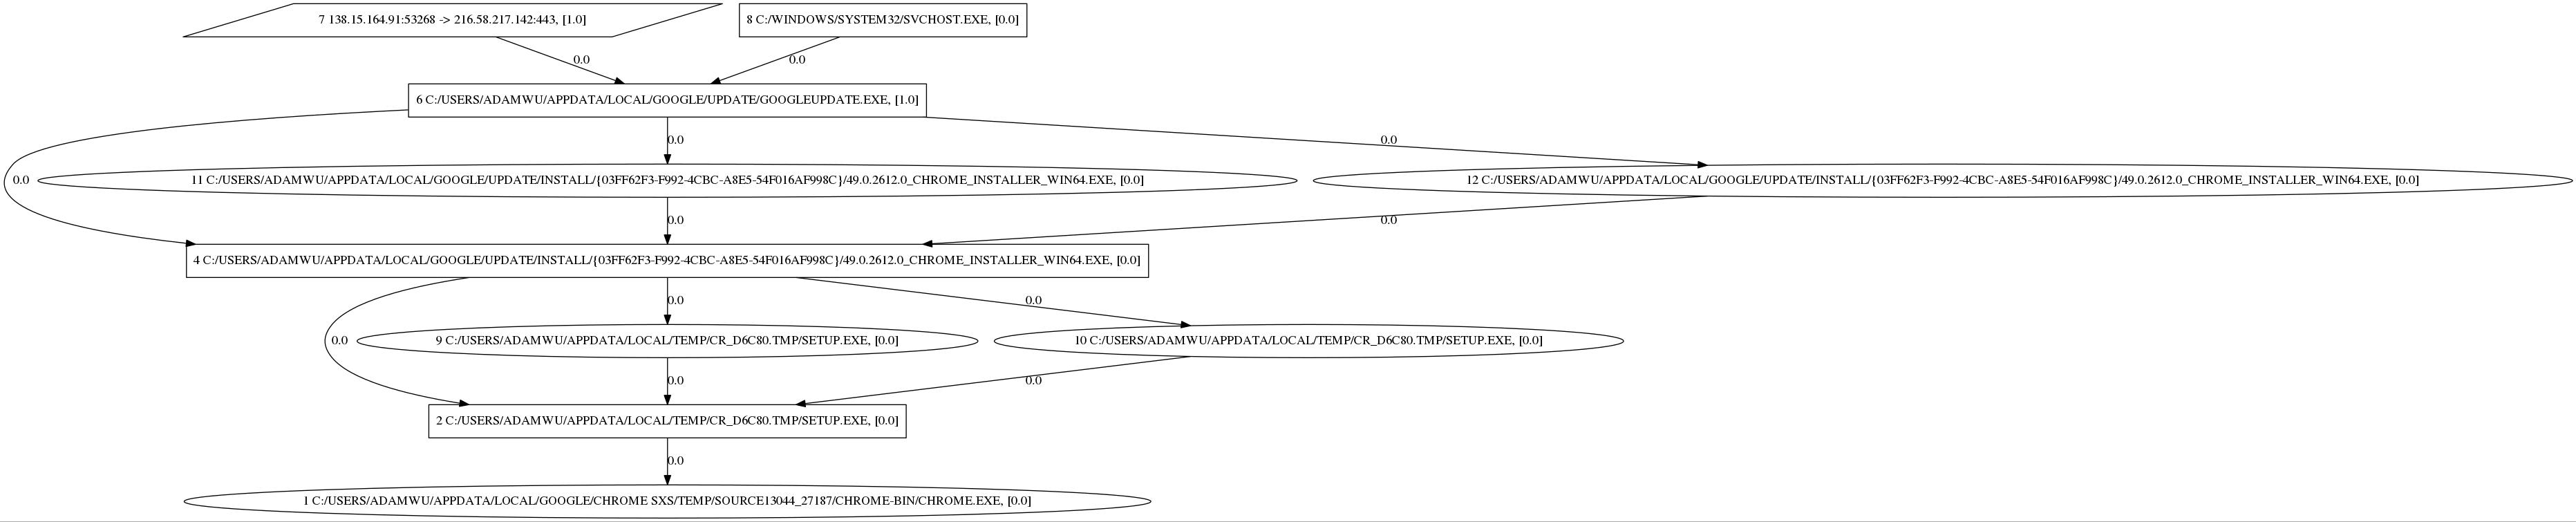
\includegraphics[width=0.5\linewidth,height=5cm]{splitTest.jpg}%
%		\label{fig:b}%
%	}%
%	\caption{The test sample of Graph Split}
%	\label{fig:sampleResult}
%\end{figure*}
\section{Approach}
In this part, we will present two parts of our work. The first one is about how to process the log file and get what kinds of information. The work flow of automatic dependency analysis is illustrated in Figure\ref{fig:steps}.
%\lipsum[1-2]
%\begin{wrapfigure}{R}{0.5\textwidth}
%	\begin{center}
%		\begin{adjustbox}{width=0.5\textwidth}
%			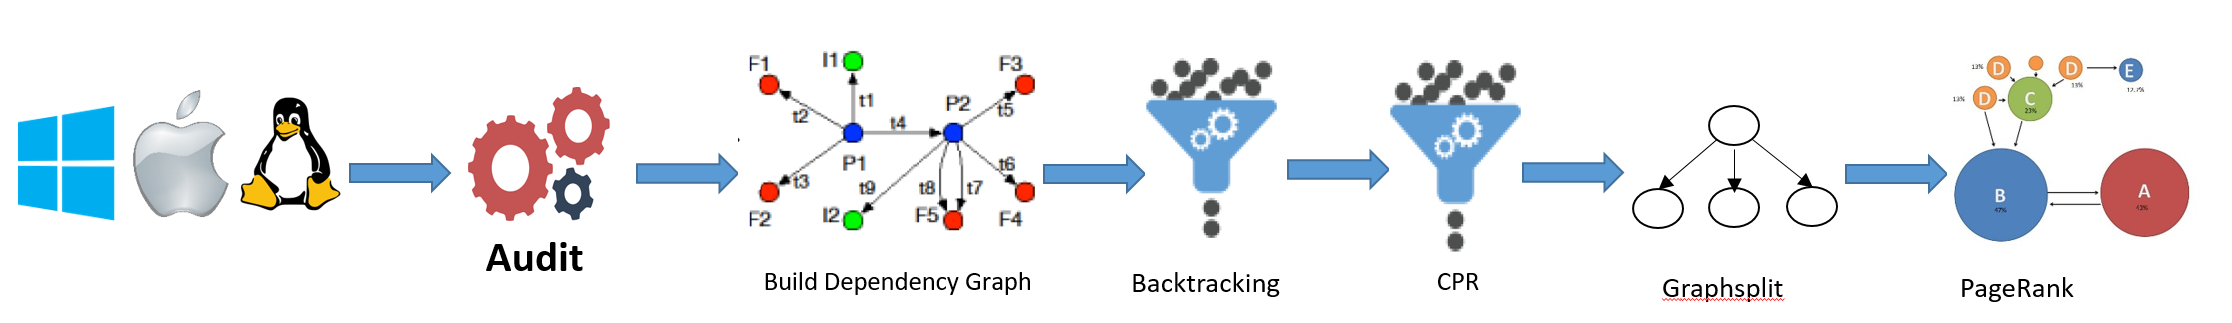
\includegraphics[clip,scale=0.35]{figFlow.png}
%		\end{adjustbox}
%	\end{center}
%\end{wrapfigure}
\begin{figure}
	\centering
	\caption{Overview of automatic dependency analysis}
	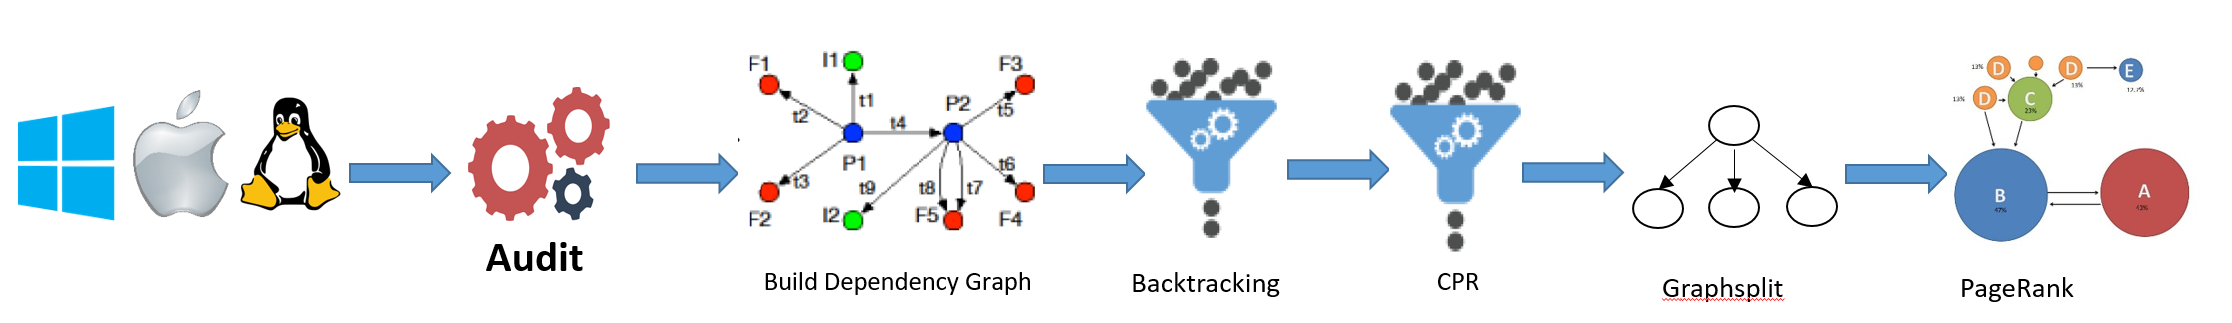
\includegraphics[width=0.48\textwidth]{figFlow.png}
	\label{fig:steps}
\end{figure}

\subsection{Enhanced Dependency Analysis (Milestone 1)}
In this section, we describe the 


\textbf{Log Parsing}.
After gathering the data, we need build the dependency graph based on the log file. There are three type vertexes representing three kind system entities: process, file and network communication.
The identifier for process is its name and id.  For file, it is identified by its absolute file path, for network communication, it is distinguished by the communication two sides' ip and port number.The attributes for these three system entities are showed in Table~\ref{mytable:table1}. We use three kind shape to represent these three system entities. According to the entities included in the system event, the parser need to process five kinds edge : process to process, process to file, file to process, network to process, process to network. The type of edge is decided by the event arguments. The output of Sysdig will use \textit{fd} as its identifier or key word. In the value part, it will use different characters to represent different objects.For example, it use \textit{f} to represent file, \textit{6} to represent IPV6 sockets,\textit{4} to represent IPV4 sockets. This kind information is necessary, without this, it is hard to know the start or end of information flow is a file or an ip address.  Through this way, the parser can know the kind of entities generating this event. For process to process event, we can directly know objects generating this event is two processes, because its event type is unique : fork or clone. In the conclusion, the parser will establish the dependency relationship between two system entities. This dependency relationship is specified by three parts: a source object, a sink object and a time interval$(t_s(e), t_e(e))$.Table2 shows the information that we collect in the log file.

\begin{table}[t!p]
	\centering
	\caption{Representation Of System Entities}
	\label{mytable:table1}
	\resizebox{0.45\textwidth}{!}{%
		\begin{tabular}{|l|c|r|}
			\hline
			Entity             & Attributes    & Shape in Graph \\ \hline
			File               & Absolute Path & Ellipse        \\ \hline
			Process            & PID and Name  & Square         \\ \hline
			Network Connection & IP and Port   & Parallelogram  \\ \hline
		\end{tabular}%
	}
\end{table}

\begin{table}[t!p]
	\centering
	\caption{Representative attributes of system events}
	\label{table2}
	\begin{tabular}{|l|c|}
		\hline
		Categories    & Attributes                    \\ \hline
		Operation     & read/write writeto fork clone \\ \hline
		Time/Sequence & Start/End Time                \\ \hline
		Argument      & IP Port data size             \\ \hline
	\end{tabular}
\end{table}

\begin{algorithm}
	\caption{GraphSplit}
	\KwIn{A dependency Graph}
	\SetKwFunction{FindPair}{FindPair}
	\SetKwFunction{UpdateGraph}{UpdateGraph}
	\SetKwFunction{RecoverTimeLogic}{RecoverTimeLogic}
	\textbf{function}: GraphSplit$(\textit(G))$\\
	$Queue$ $\leftarrow$ \FindPair{$G$}\;
	\While{Queue is not Empty}{
		$V$ $\leftarrow$ $Queue.poll()$\;
		$S \leftarrow V.source$\;
		$T \leftarrow V.target$\;
		\If{Set contains S $or$ Set contains T}{continue}
		$list1 \leftarrow$ list of outgoing edges of $S$ whose object is not $T$\;
		$list2 \leftarrow$ V.list\;
		\UpdateGraph($G$,$list1$,$list2$)\;
		add $S$ to Set\;
		$Queue \leftarrow$ \FindPair($G$)\;
	}
	\RecoverTimeLogic{$Set$}\;	
	\label{alg:split}
\end{algorithm}

\textbf{Limitations of Existing Work}.
In the existed research work, the information for the dependency analysis only includes file name, process, IP addresses and attributes of events including event origins, operations $($file read/write$)$, and other security-related properties. However, to infer application reputation, only these attributes are not enough.
The reason is that they are mainly used to form a dependency graph with nodes being entities and edges representing data flows;
but to infer reputations, each edge carries different weights in impacting the reputation propagation as shown in Figure~\ref{fig:steps}.
Moreover, dependency analysis includes filters based on the existing works~\cite{backtracking,backtracking2}, which are not optimized for inferring reputations.
Therefore, it is \emph{necessary} to collect more attributes for the purpose of assigning weights to edges in the produced dependency graph and include more specialized filters to filter out unrelated events in the graph. 

\textbf{Relative Time to the POI event}.
Currently, we finished the building the dependency graph with additional necessary information. The first one is the relative time to the POI event(Detection Point).Once an application or a library is introduced to a system, it may get modifications via application updates, manually customizations, or malicious alternations. 
That is, a file node in the dependency graph can have multiple \emph{write} edges $($incoming edges$)$ representing initial creation and subsequent updates.
Intuitively, the write comes latter carries more weights in impacting the application reputation.
%For example, an application could be created by a benign program and latter gets altered by a malicious program; to capture the latter malicious alternation, usually injecting malicious code, the application's reputation should be considered as \emph{more towards malicious}. 
Therefore, \emph{the time when an event occurs} is one factor that impacts the reputation propagation: the latter it happens, the more weight it carries.
As such, given a POI event, we propose to compute \emph{the relative time to the start time of the POI event} for each of the subsequent edges included into the dependency graph,
and use this new attribute as part of the computation for the weights of the edges. 

\textbf{Amount of Transfered Data}.
The second  improvement compared with the traditional dependency analysis method is that we observe that the amount of transferred data is another important factor that impacts the reputation propagation.Not all the updates are rewriting application executables to malicious executables; some updates to an application are merely for property updates.
For example, in Windows, the search indexer program frequently updates executables' metadata for indexing purposes, and each update writes only a few bytes to the executables.
Therefore, we propose to extract \emph{the amount of data transferred} for each read/write operation and annotates the corresponding edges in the dependency graph with this information.
The larger amount of data transferred, the more important the edge is.

\begin{algorithm}
	\caption{FindPair}
	\KwIn{A dependency Graph(G)}
	\KwResult{A queue containing the vertex pair need to be splited}
	\textbf{function}: FindPair$\textit(G)$\\
	$V \leftarrow G.vertexSet$\;
	\For{$v \in V$}{
		$E \leftarrow$ incoming edges of $v$\;
		\If{$\exists e \in E$ sharing the same source}{
			$vertexPair.source \leftarrow e.source$\;
			$vertextPair.object \leftarrow v$\;
			$vertexPair.object.list$ add $e$\; 
			$Queue$ add $vertexPair$\;}
	}
	\Return{Queue}
\end{algorithm}



\begin{table*}[!hp]
	\centering
	\caption{Statistical Result}
	\label{my-label}
	%	\resizebox{0.5\textwidth}{!}{%
	\begin{scriptsize}
		\begin{tabular}{|l|r|r|r|r|r|r|r|}
			\hline
			sample                    & log file size & vertex(original) & edge(original) & vertex(backtracking) & edge(backtracking) & vertex(CPR) & edge(CPR) \\ \hline
			apt-get instll unrar      & 17.5MB        & 5092             & 28502          & 2148                 & 3911               & 2148        & 2346      \\ \hline
			apt-get instll postgresql & 53.0MB        & 12174            & 82684          & 2667                 & 11564              & 2667        & 3178      \\ \hline
			apt-get install zookeeper & 19.7MB        & 4264             & 24368          & 2516                 & 6982               & 2516        & 3020      \\ \hline
			apt-get install mongoDB   & 65.9MB        & 4205             & 45510          & 2712                 & 11131              & 2712        & 2949      \\ \hline
			apt-get install wireshark & 66.2MB        & 5838             & 64411          & 3511                 & 34136              & 3511        & 4488      \\ \hline
		\end{tabular}%
	\end{scriptsize}
	
	%	}
\end{table*}

\begin{algorithm}
	\caption{UpdateGraph}
	\KwIn{A dependency Graph and.\\
		list1 is a list of outgoning edges of the source except edges whose object is V. \\
		list2 is a list containing edges between S and V}
	\textbf{function}: UndateGraph$\textit(G, list1, list2)$\\
	$list \leftarrow$ empty list of vertex\;
	\For{$ e \in list2$}{
		$u \leftarrow split(S)$\;
		$list$ add $u$\;
		$G$ add $u$\;
		$G$ add a new edge from $u$ to $V$\;
	}
	\For{$u \in list$}{
		\For{$e \in list1$}{
			$G$ add a new edge from $u$ to the object of $e$\;}
	}
	\For{$u \in list$}{
		\For{$e \in$ in the incoming edges of $S$}{
			$G$ add a new edge from the source of $e$ to $u$\;}
	}
	remove $S$, the incoming and outgoing edges of $S$ from the $G$\;	
\end{algorithm}



\subsection{Inference of Application Reputation via PageRank (Milestone 2)}
PageRank~\cite{pagerank} considers the World Wide Web as a set of linked nodes and ranks them based on their importance. The insight of PageRank is that a node linked by important nodes should be more important than the ones linked by uninfluenced nodes. That is, a web page's "reputation" is impacted by all the other web pages pointing to it. PageRank uses a transition matrix to represent the weights of edges from node \textit{j} to node \textit{i}. However,although Causality Preserve Reduction can merge many edges, there still may have multiple edges existing the same pair of nodes, because we don't want that the dependency relationship is lost during Causality Preserve Reduction. Therefore, we borrow the idea of static single assignment from(SSA)~\cite{nielson2004principles}, splitting source node  into multiple nodes, where each of the split node has only one outgoing edge pointing to target node. We need duplicate all the edges originally pointing to source to each of the split node from node j.By replacing source node with the split nodes, we can then use PageRank to compute system entities' reputation.

\textbf{Graph Split}.
Algorithm~\ref{alg:split} shows the algorithm for GraphSplit. 
The basic idea for GraphSplit is that for every vertex$(V)$ of the dependency graph, we need to check its incoming edges. If several incoming edges share the same source, we declare a \textit{vertexPair} contains object $V$, source $S$ and a list of edges that connect these two vertexes. We maintain a queue for all $vertexPairs$. We also maintain a set of vertex has already been split.If we find the current $vertexPair.S$ or $vertexPair.V$ is split, then we just skip it in current round. We will split it in the next round. Here is the relevant function of GraphSplit.

\begin{algorithm}
	\caption{RecoverTimeLogic}
	\KwIn{A set of splited vertex}
	\textbf{function}: RecoverTimeLogic$\textit(Set)$\\
	$V \leftarrow G.vertexSet()$\;
	\For{$v \in V$}{
		\If{$v$ is the splitting node belongs to $Set$}{
			$endtime \leftarrow$ the biggest endtime of outgoing edges of $v$\;
			\For{$e \in$ incoming edges of v}{
				\If{$e.start > endtime$}{remove this edge\;
				}
			}
		}
	} 	
\end{algorithm}

%\begin{algorithm}
%	\caption{RecoverTimeLogic}
%	\KwIn{A set of splited vertex}
%	\textbf{function}: RecoverTimeLogic$\textit(Set)$\\
%	$V \leftarrow G.vertexSet()$\;
%	\For{$v \in V$}{
%		\If{$v$ is the splitting node belongs to $Set$}{
%			$endtime \leftarrow$ the biggest endtime of outgoing edges of $v$\;
%			\For{$e \in$ incoming edges of v}{
%				\If{$e.start > endtime$}{remove this edge\;
%				}
%			}
%		}
%	} 	
%\end{algorithm}



\section{Preliminary Result}
%\begin{figure*}[htp] 
%	\centering
%	\subfloat[original graph]{%
%		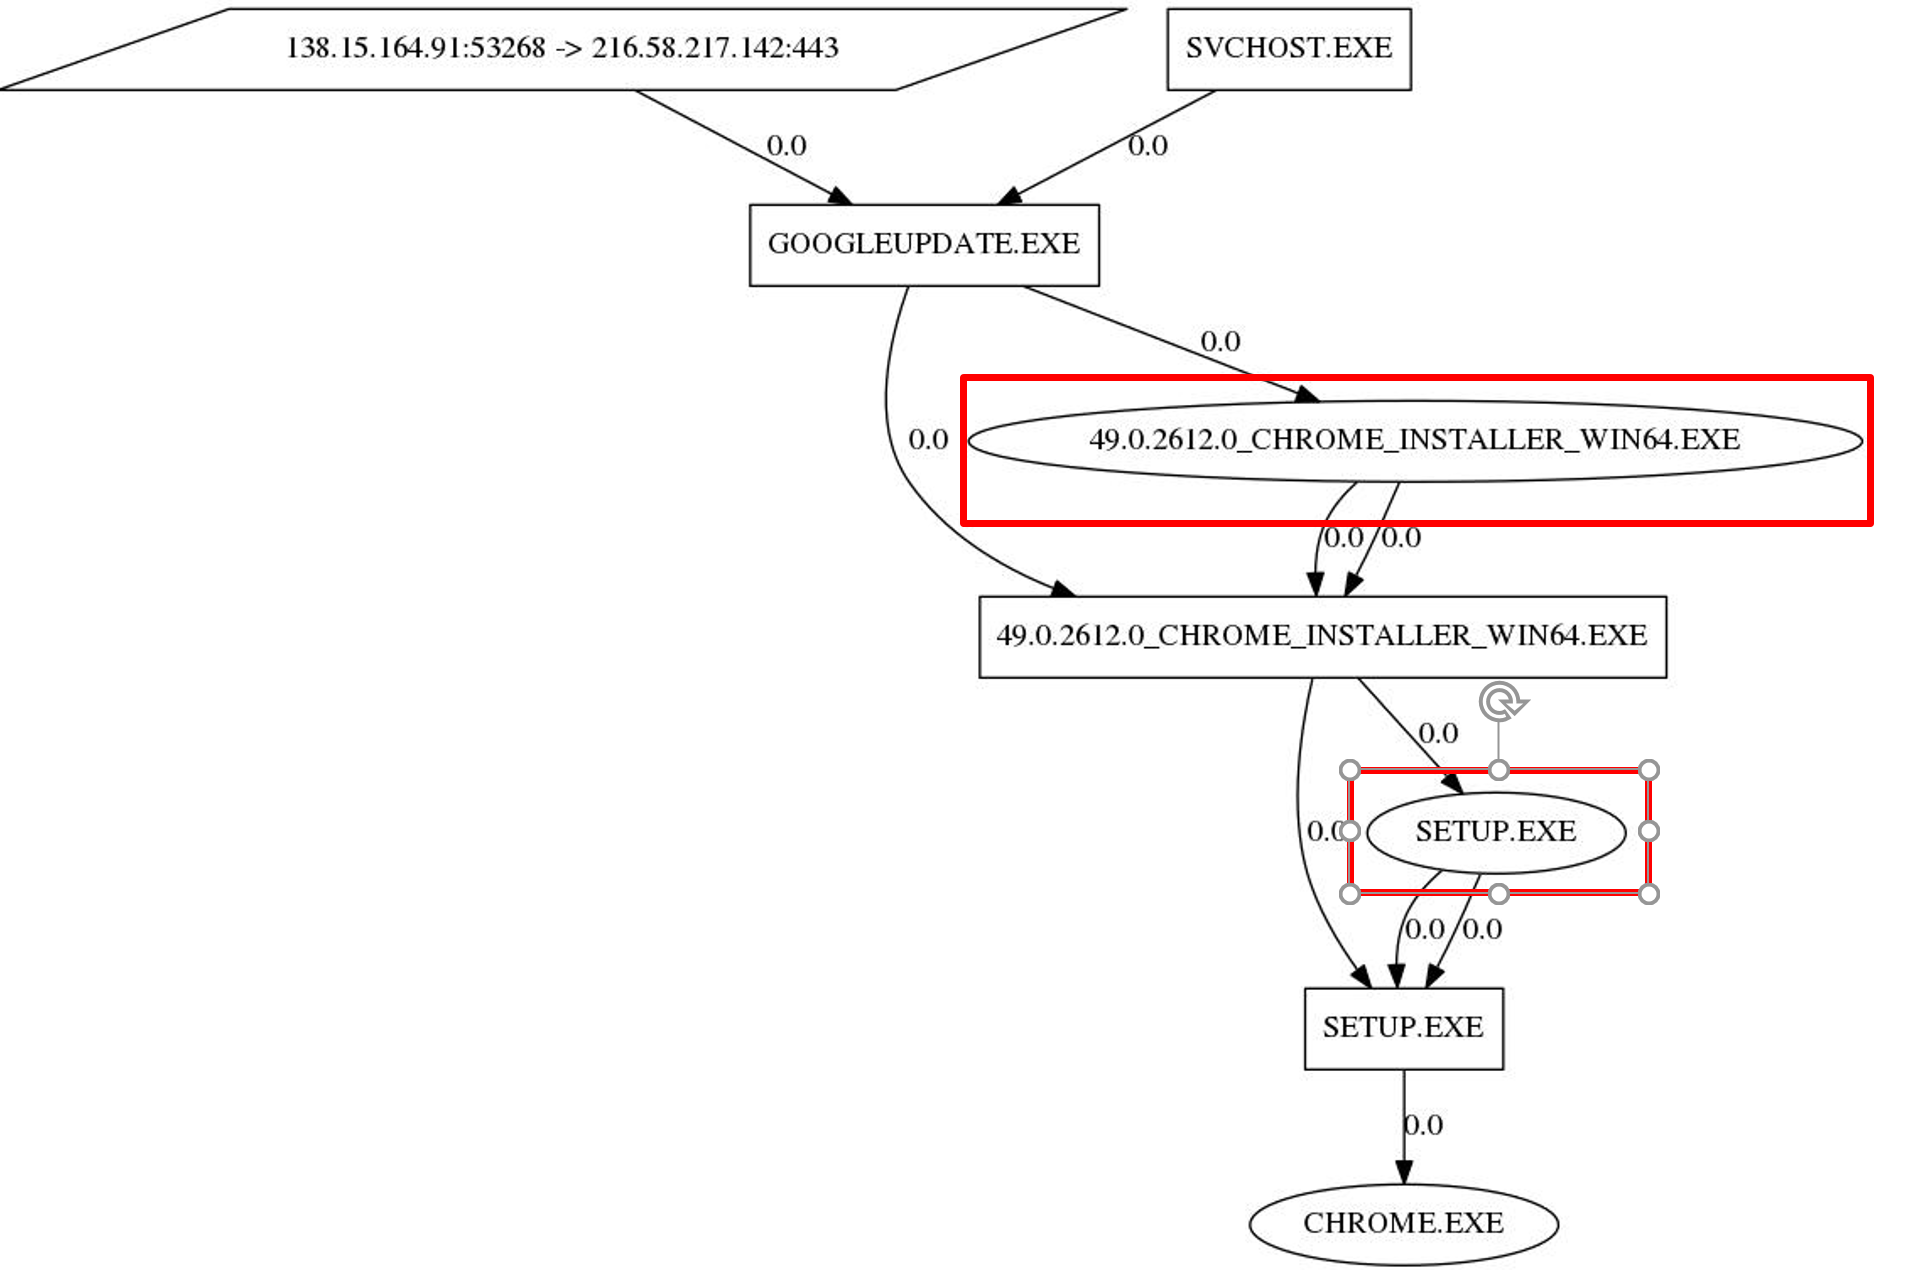
\includegraphics[width=0.5\linewidth,height=5cm]{testSample.png}%
%		\label{fig:a}%
%	}%
%	\hfill%
%	\subfloat[after splitting]{%
%		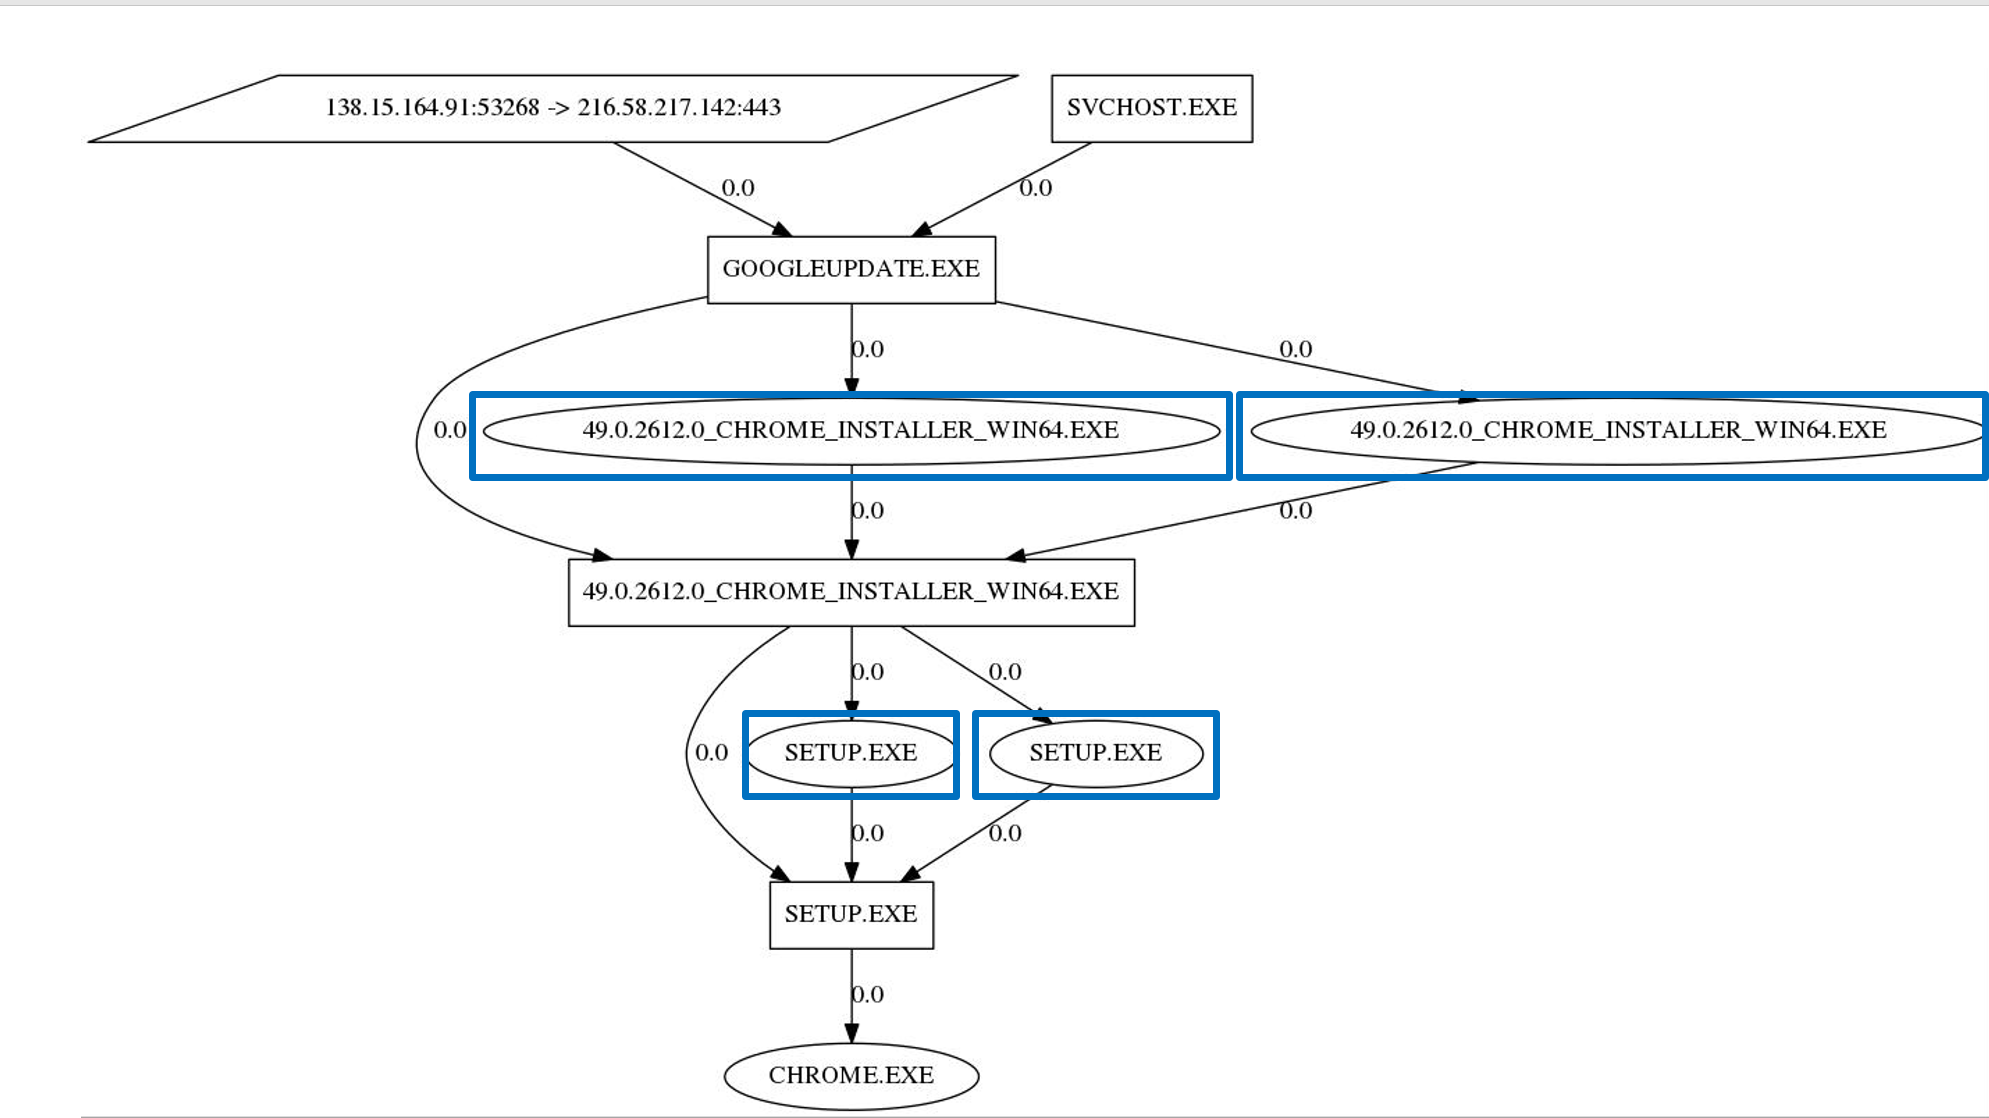
\includegraphics[width=0.5\linewidth,height=5cm]{sampleResult.png}%
%		\label{fig:b}%
%	}%
%	\caption{The test sample of Graph Split}
%	\label{fig:sampleResult}
%\end{figure*}

In this part, we will show our current project progress. The first table show our method's performance on the system monitoring data. The first column show the test case is that user use Linux command: \textit{apt get} to install some applications. This operation is quite common in different environment. The second column is the log file size. We use the vertex and edge number to evaluate the size of the dependency graph. It is very obvious that our method reduce the number of vertex and edge in the dependency graph.  It reduce the burden for further calculation. We also already test out GraphSplit on a small sample from the real-world scenario.Figure~\ref{fig:splitsample} and Figure~\ref{fig:splitresult} is the sample and result of GraphSplit. The node in the red square has multiple edges pointing to the same object, so this one need to be split. The node in the blue square is nodes generated by Graphsplit algorithm. In the next step, we will gather the aduiting data in a longer time and test its performance and overheat. 
%\begin{table*}
%	\centering
%	\caption{The size of log file and dependency graph}
%	\begin{tabular}{ |l|c|c|c|c|c|c|r| }{\textwidth}
%		\hline
%		apt-get Install unrar & log file size & vertex number $(origina)$ & edge number $(Orignal)$ & vertex number$(Backtracking)$ & edge number$(Backtracking)$ & vertex number $(CPR)$ & edge number$(CPR)$\\
%		\hline
%	\end{tabular}
%\end{table*}


\begin{figure}
	\centering
	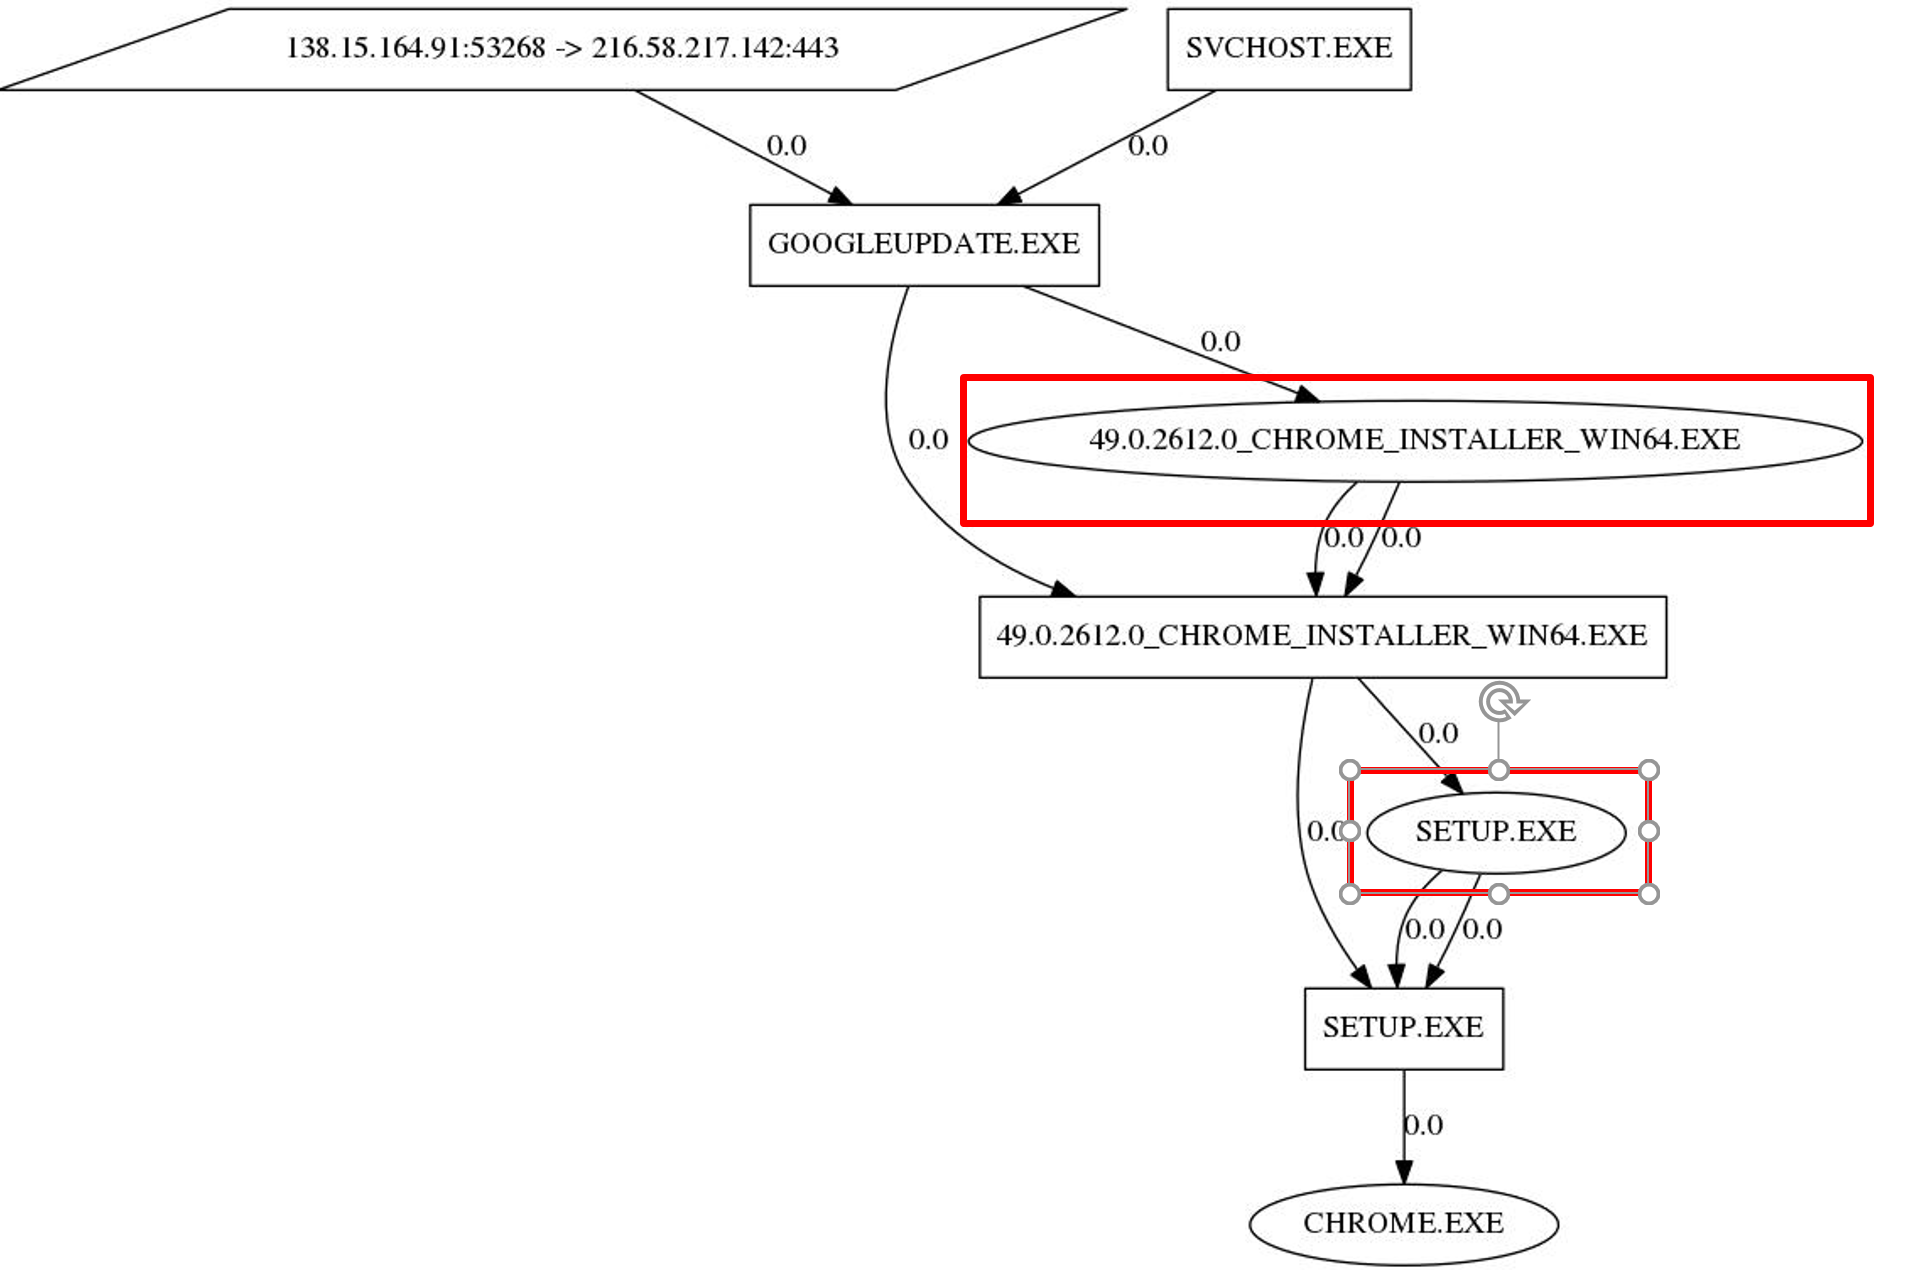
\includegraphics[width=0.5\textwidth]{testSample.png}
	\caption{Test sample}
	\label{fig:splitsample}
\end{figure}
\begin{figure}
	\centering
	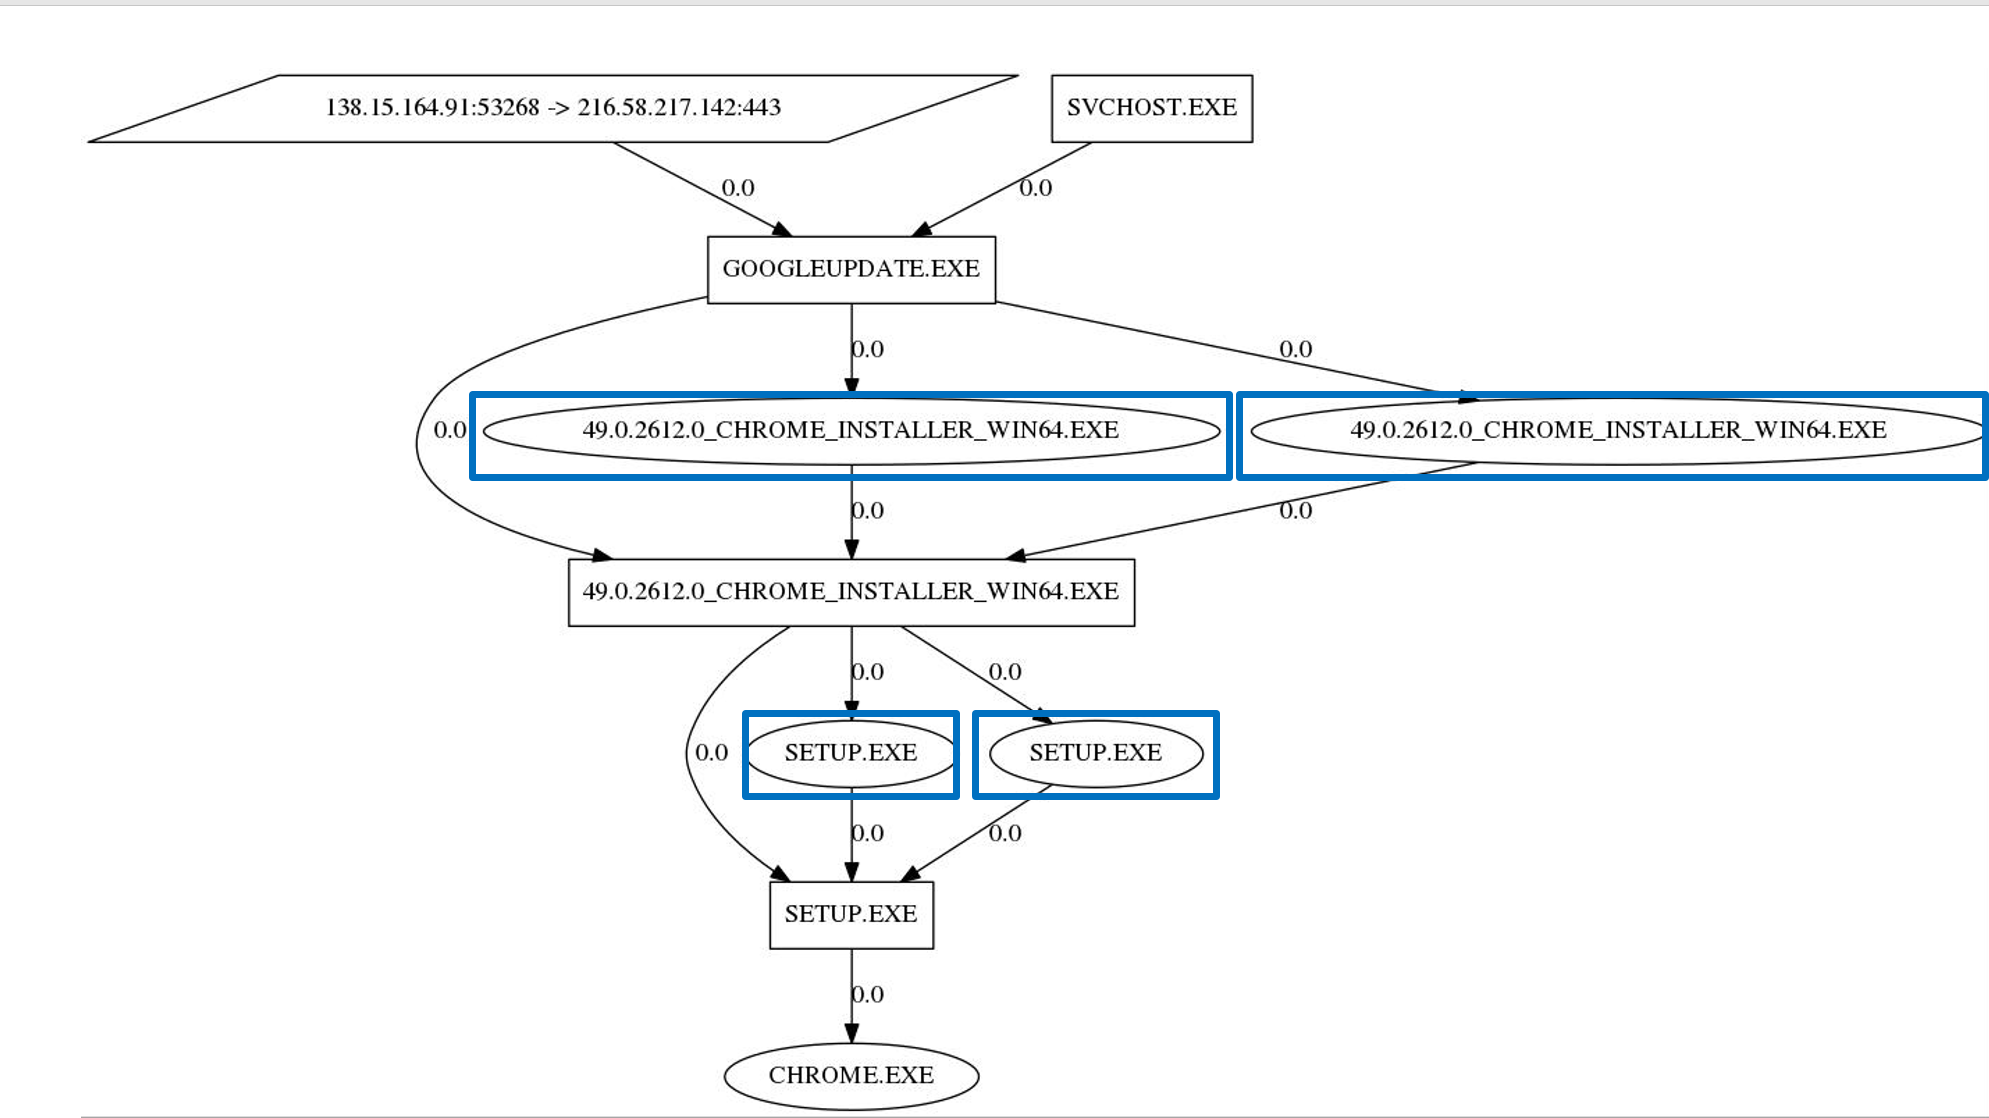
\includegraphics[width=0.5\textwidth]{sampleResult.png}
	\caption{GraphSplit Result}
	\label{fig:splitresult}
\end{figure}
\vspace{2cm}
%\begin{figure}[!htbp]
%	\begin{minipage}[t][0.8\textheight]{0.5\textwidth}
%		\centering
%		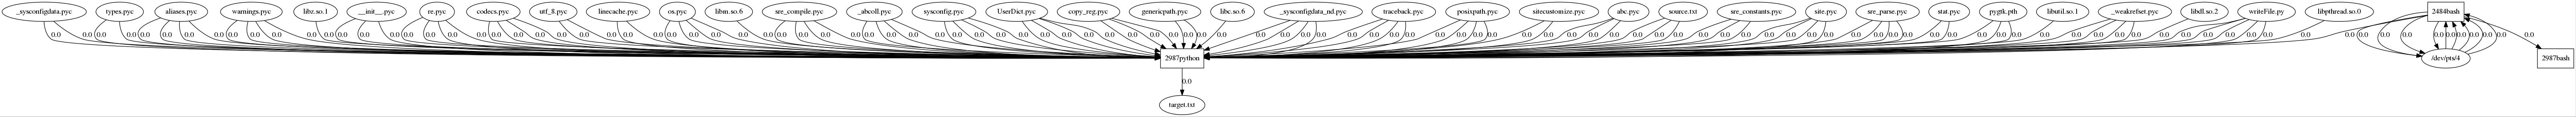
\includegraphics[align=c, width=\textheight,angle=90]{fileBack.jpg}
%		\hspace{0.1\textwidth}
%		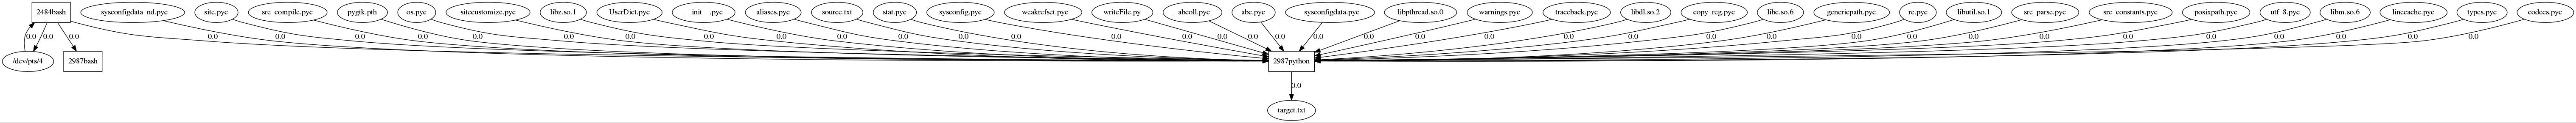
\includegraphics[align=c, width=\textheight,angle=90]{fileCPR.jpg}
%	\end{minipage}
%	\caption{Backtracking And Causality Preserve Reduction Result}
%	\label{fig:backandCPR}
%\end{figure}




%\section{Evaluation}
%In this part, will show our current project progress. The first table show our method's performance on the system monitoring data. It is very obvious that our method reduce the number of vertex and edge in the dependency graph. It reduce the burden for further calculation. We also already test out GraphSplit on a small sample from the real-world scenario. Figure\ref{fig:sampleResult} is the result of GraphSplit. In the next step, we will gather the aduiting data in a longer time and test its performance and overheat. 
%\begin{table*}
%	\centering
%	\caption{The size of log file and dependency graph}
%	\begin{tabular}{ |l|c|c|c|c|c|c|r| }{\textwidth}
%		\hline
%		apt-get Install unrar & log file size & vertex number $(origina)$ & edge number $(Orignal)$ & vertex number$(Backtracking)$ & edge number$(Backtracking)$ & vertex number $(CPR)$ & edge number$(CPR)$\\
%		\hline
%	\end{tabular}
%\end{table*}

%\begin{table}[]
%	\centering
%	\caption{Statistical Result}
%	\label{my-label}
%	\resizebox{0.5\textwidth}{!}{%
%		\begin{tabular}{|l|r|r|r|r|r|r|r|}
%			\hline
%			sample                    & log file size & vertex(original) & edge(original) & vertex(backtracking) & edge(backtracking) & vertex(CPR) & edge(CPR) \\ \hline
%			apt-get instll unrar      & 17.5MB        & 5092             & 28502          & 2148                 & 3911               & 2148        & 2346      \\ \hline
%			apt-get instll postgresql & 53.0MB        & 12174            & 82684          & 2667                 & 11564              & 2667        & 3178      \\ \hline
%			apt-get install zookeeper & 19.7MB        & 4264             & 24368          & 2516                 & 6982               & 2516        & 3020      \\ \hline
%			apt-get install mongoDB   & 65.9MB        & 4205             & 45510          & 2712                 & 11131              & 2712        & 2949      \\ \hline
%			apt-get install wireshark & 66.2MB        & 5838             & 64411          & 3511                 & 34136              & 3511        & 4488      \\ \hline
%		\end{tabular}%
%	}
%\end{table}
%\begin{figure*}[htp] 
%	\centering
%	\subfloat[original graph]{%
%		\includegraphics[width=0.5\linewidth,height=5cm]{sampleBeforeSplit.jpg}%
%		\label{fig:a}%
%	}%
%	\hfill%
%	\subfloat[after splitting]{%
%		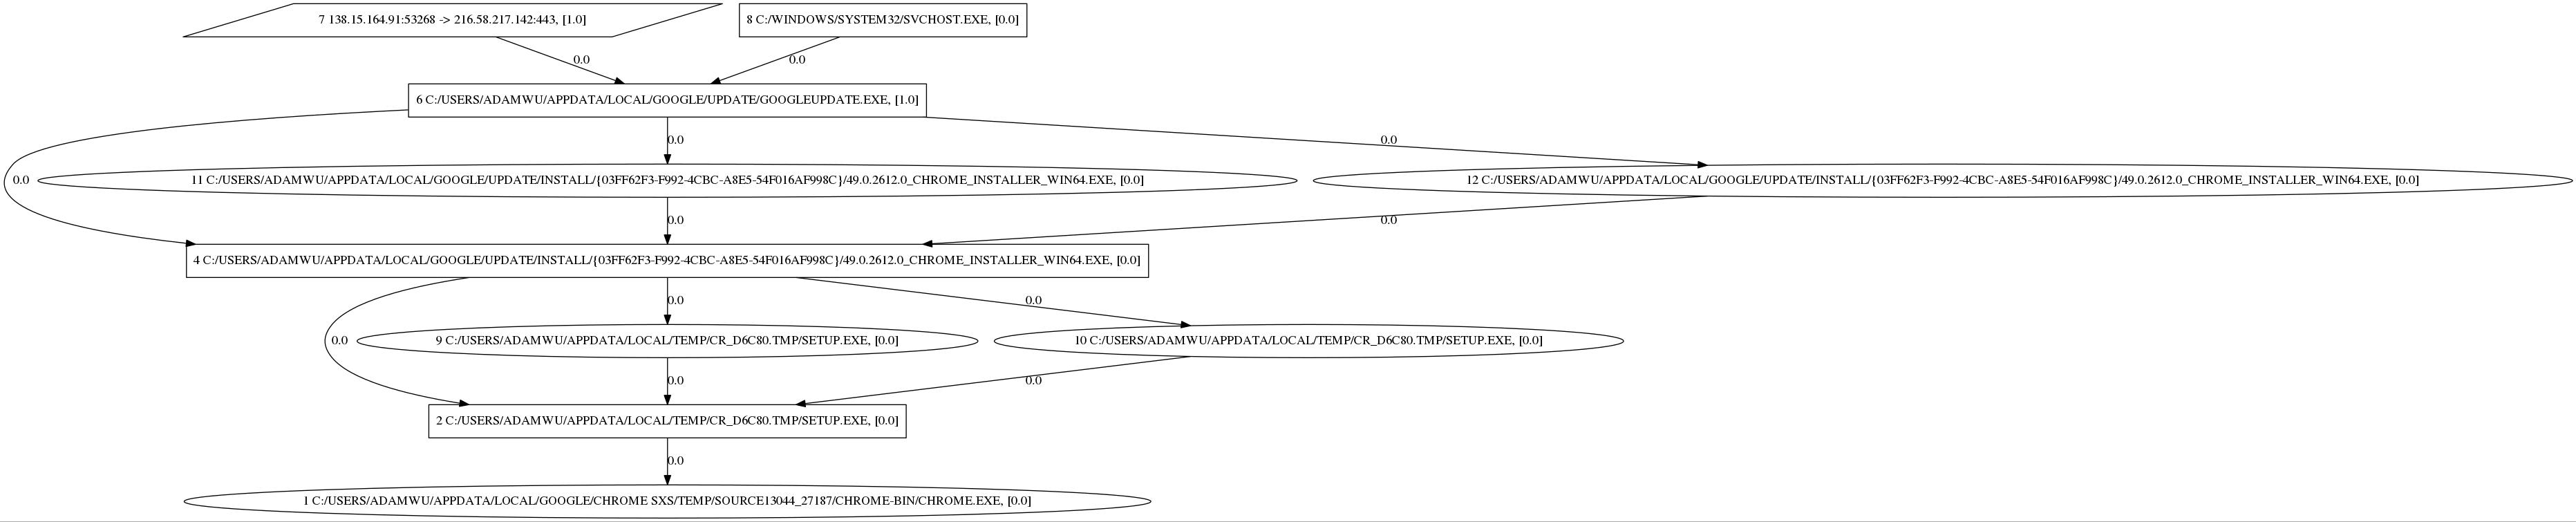
\includegraphics[width=0.5\linewidth,height=5cm]{splitTest.jpg}%
%		\label{fig:b}%
%	}%
%	\caption{The test sample of Graph Split}
%	\label{fig:sampleResult}
%\end{figure*}









% end the environment with {table*}, NOTE not {table}!
\bibliographystyle{abbrv}
\bibliography{sigproc}  % sigproc.bib is the name of the Bibliography in this case


\end{document}
